%!TEX root = ../../../../memoria.tex
\subsection{\accountsEF}

	Permite agregar o quitar permisos a los usuarios. El sistema actualmente permite crear usuarios y modificar sus permisos permitiendo o eliminando las componentes relacionadas a sus permisos.

	\begin{figure}[H]
		\centering
		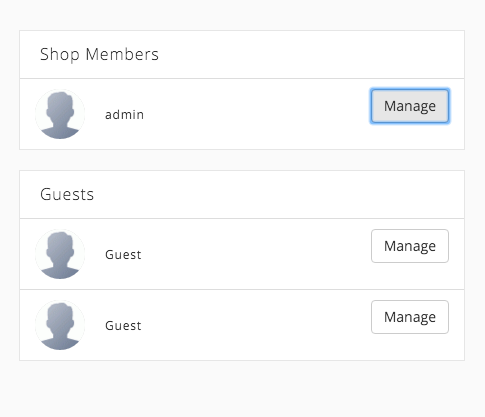
\includegraphics[width=0.6\textwidth]{figuras/dashboard/account/users.png}
		\caption{Interfaz con los usuarios del sistema.}
		\label{figure:dashboard:account:users}
	\end{figure}


	\begin{figure}[H]
		\centering
		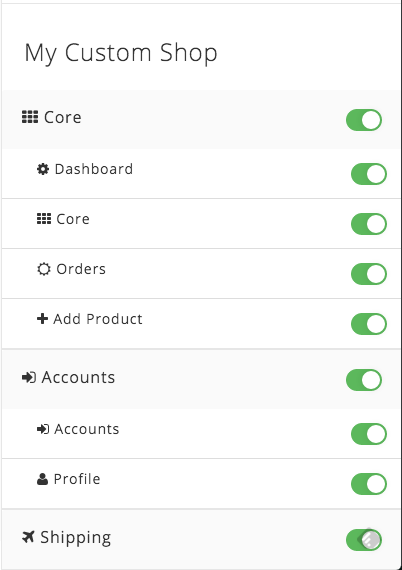
\includegraphics[width=0.6\textwidth]{figuras/dashboard/account/permisos.png}
		\caption{Interfaz para administrar los permisos del sistema.}
		\label{figure:dashboard:account:permisos}
	\end{figure}

\begin{table}[H]
    \centering
	\begin{tabular}{ |l|c||l| }
		\hline Campo & Requerido & Restricción \\ \hline
		\multirow{1}{*}{\textit{Core}} 			&  \checkmark 	& Boolean \\ \hline
		\multirow{1}{*}{\textit{Dashboard}} 	&  \checkmark	& Boolean \\ \hline
		\multirow{1}{*}{\textit{Orders}} 		&  \checkmark	& Boolean \\ \hline
		\multirow{1}{*}{\textit{Add Product}} 	&  \checkmark	& Boolean \\ \hline
		\multirow{1}{*}{\textit{Accounts}} 		&  \checkmark	& Boolean \\ \hline
		\multirow{1}{*}{\textit{Profile}} 		&  \checkmark	& Boolean \\ \hline
		\multirow{1}{*}{\textit{Shipping}} 		&  \checkmark	& Boolean \\ \hline
	\end{tabular}
 	\caption{Resumen restrincciones formulario para los permisos.}
    \label{tab:dashboard:account:form:restrictions:account}
\end{table}